\chapter{Introduction} \label{chap:introduction}

Pneumonia is swelling (inflammation) of the tissue in one or both lungs. It is usually formed at the end of breathing tubes of the lungs and cause these tubes to inflame and fill up with fluid. In the UK, pneumonia effects around 8 in 1000 adults each year \cite{nhs}. Global economic cost of pneumonia has estimated at \$17 billion annually \cite{cost}. Currently detecting pneumonia cases heavily relies on chest X-ray image examination which requires expert radiologists to diagnose. Building intelligent system to diagnose the pneumonia can help  health care services to increase efficiency, reduce costs and could help increase early diagnoses in countries with inadequate access to healthcare.

\section{Related work}

There are number of research has been published about lung diseases related detection. Most preeminent ones are the CheXNet \cite{CheXNetRP} and ChestX-ray8 \cite{ChestX-ray8}, both of these research carried out by training on same dataset ChestX-ray8 \cite{ChestX-ray8}. ChestX-ray8 comprises of approximately 100,000 frontal view chest X-ray images labelled by extracting information from the accompanied radiologists notes with using variety of different NLP (Natural language processing) techniques from the OpenI\cite{openi} database. ChestX-ray8 authored by researchers from National Institute of Health (NIH) and published at 2018.
Most profound effect of this paper is the creation of the ChestX-ray8 dataset which has become one of the widely used dataset in computer vision research related to lung diseases. More detailed information about the dataset can be found in dataset section of this proposal. 

CheXNet is another related article authored by researchers from Stanford University ML group. Prediction of lung diseases achieved by 121 layer convolutional neural network and designed to predict 14 pathologies in the ChestX-ray8 dataset. One of the major importance of this paper is the setting the setting benchmark for human level detection for chest X-ray images. One of the most fundamental difference of the X-ray related disease prediction is the definition of human level accuracy. Due to the nature of required expertise in X-ray images leaves general public out of the scope when it comes to human level performance of these pathologies. Anyone who have not been trained in radiology will not be able to detect any lung diseases in the Chest X-ray images. For example the image below is sample of two chest X-ray images almost indistinguishable to general audience.

\begin{figure}[H]%
    \centering
    \subfloat{{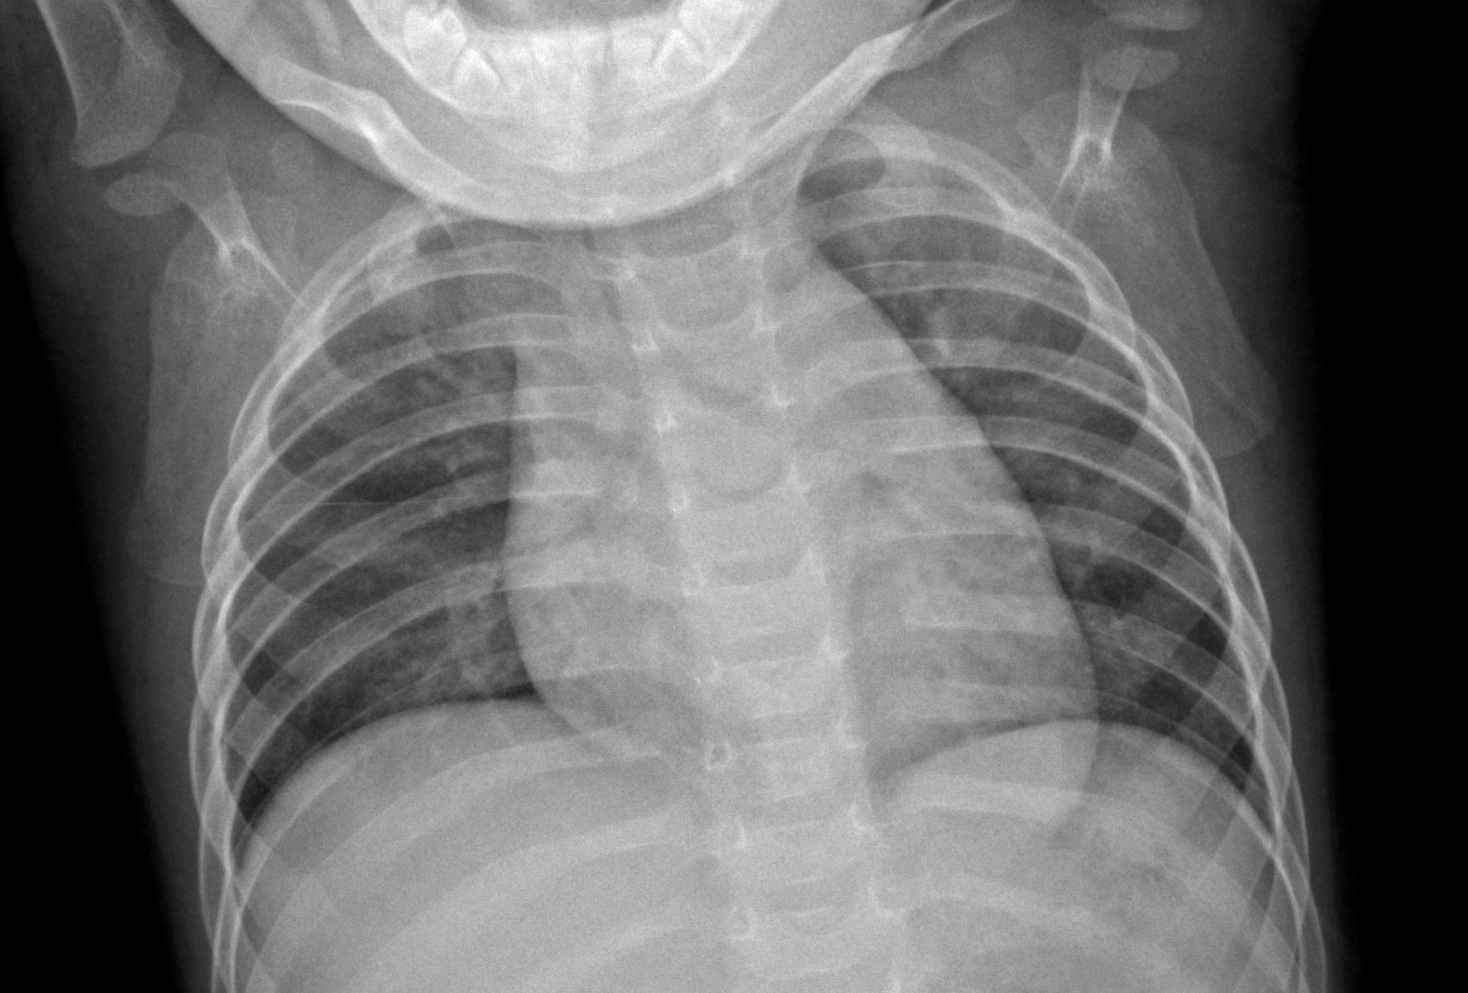
\includegraphics[width=.4\textwidth]{img/chest_xray_train_NORMAL_IM-0133-0001.jpeg} }}%
    \qquad
    \subfloat{{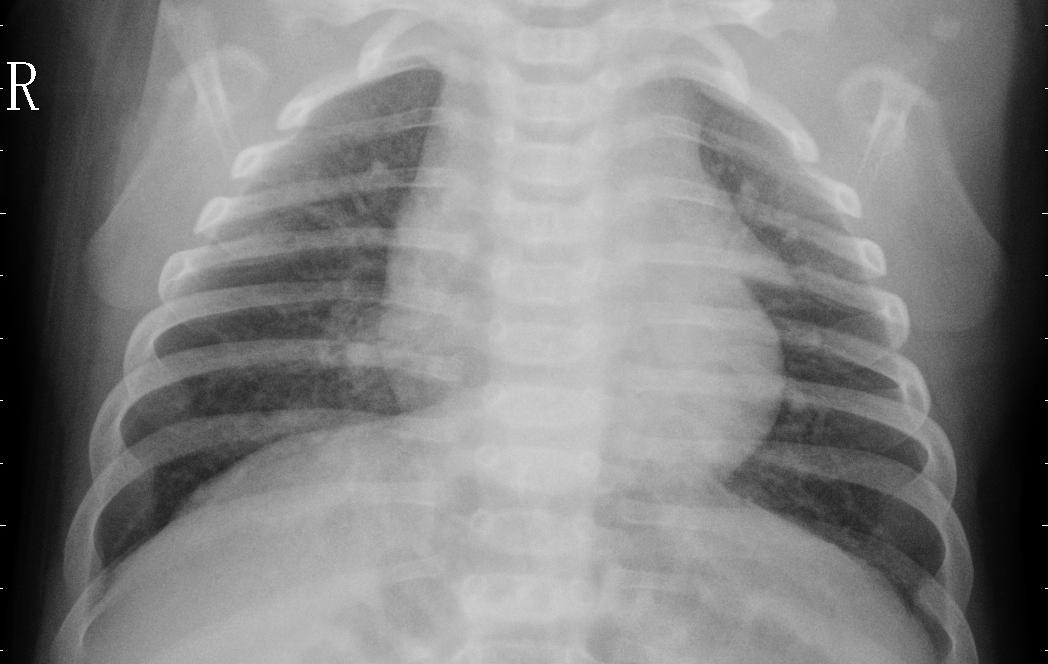
\includegraphics[width=.4\textwidth]{img/chest_xray_train_PNEUMONIA_person1007_virus_1690.jpeg} }}%
    \caption{Two sample X-ray Chest images with and without pneumonia.}%
    \label{fig:sample}%
\end{figure}
Given this challenge authors of the CheXNet conduct a test to establish benchmark for radiologists. They have collected 420 frontal chest X-rays and asked practicing radiologists in Stanford University to label them for all 14 pathologies. Radiologists selected with different range of experience, and had 4, 7, 25 and 28 years of experience. X-ray images presented to radiologists without any patient information or any symptoms experienced by patients and their diagnoses predictions measured based on underlying state of the X-ray patients. Fallowing is the table showing the summary statistic of this test for the 4 radiologists participated to test on F1 score, which is harmonic average of precision and recall.\cite{CheXNetRP}:
\begin{table}[h!]
    \centering
     \begin{tabular}{l r} 
     \hline
      & F1 Score (95\% CI) \\ [0.5ex] 
     \hline
     Radiologists 1 & 0.383 (0.309, 0.453) \\ 
     Radiologists 2 & 0.356 (0.282, 0.428) \\
     Radiologists 2 & 0.365 (0.291, 0.435) \\
     Radiologists 4 & 0.442 (0.390, 0.492) \\
     \hline
     Radiologists Avg & 0.387 (0.330, 0.442) \\ [1ex] 
     \hline
     \end{tabular}
     \caption{Radiologist prediction performances from CheXNet \cite{CheXNetRP}.}
     \label{table:radiologist}
\end{table}

Importance of this test is that it gives us a rough estimate for human level accuracy benchmark to assess the model performance for new detection models.
\clearpage